%!TEX TS-program = Xelatex  
%!TEX encoding = UTF-8 Unicode  
  
  
\documentclass[12pt]{article}  
\usepackage{geometry}  
\geometry{letterpaper}  
  
\usepackage{fancyhdr} 
\usepackage{layout}
\addtolength{\hoffset}{-1.0cm} \addtolength{\textwidth}{2cm}
\addtolength{\voffset}{-1.0cm} \addtolength{\textheight}{2cm}
\usepackage[rgb]{xcolor}

\usepackage{cite}
\makeatletter
\def\@cite#1#2{\textsuperscript{[{#1\if@tempswa , #2\fi}]}}
\makeatother

\usepackage{listings}
\definecolor{dkgreen}{rgb}{0,0.6,0}
\definecolor{gray}{rgb}{0.5,0.5,0.5}
\definecolor{bcol}{rgb}{0.85,0.85,0.85}
\definecolor{mauve}{rgb}{0.58,0,0.82}
\definecolor{mygray}{gray}{.9}
\definecolor{mypink}{rgb}{.99,.91,.95}
\definecolor{mycyan}{cmyk}{.3,0,0,0}
\usepackage{cite} 
\newcommand{\ucite}[1]
{\textsuperscript{\cite{#1}}}

\lstset{ %
language=python,                % the language of the code
basicstyle=\footnotesize,       % the size of the fonts that are used for the code
numbers=left,                   % where to put the line-numbers
numberstyle=\tiny\color{gray},  % the style that is used for the line-numbers
stepnumber=1,                   % the step between two line-numbers. If it's 1, each line
                                % will be numbered
numbersep=5pt,                  % how far the line-numbers are from the code
backgroundcolor=\color{bcol},   % choose the background color. You must add \usepackage{color}
showspaces=false,               % show spaces adding particular underscores
showstringspaces=false,         % underline spaces within strings
showtabs=false,                 % show tabs within strings adding particular underscores
frame=shadowbox,                % adds a frame around the code
rulecolor=\color{black},        % if not set, the frame-color may be changed on line-breaks within not-black text (e.g. commens (green here))
tabsize=2,                      % sets default tabsize to 2 spaces
captionpos=t,                   % sets the caption-position to bottom
breaklines=true,                % sets automatic line breaking
breakatwhitespace=false,        % sets if automatic breaks should only happen at whitespace
title=\lstname,                     % show the filename of files included with \lstinputlisting;
                                    % also try caption instead of title
keywordstyle=\color{blue},          % keyword style
commentstyle=\color{dkgreen},       % comment style
stringstyle=\color{mauve},          % string literal style
escapeinside=``,                    % if you want to add LaTeX within your code
morekeywords={LONG64,LONGLONG,bool}                % if you want to add more keywords to the set
}



\usepackage{flushend, cuted} %

\usepackage{indentfirst,latexsym,bm}
\usepackage{amsmath,amssymb,amsfonts}
\usepackage{pifont} 
\usepackage{fontspec,xltxtra,xunicode}  
\defaultfontfeatures{Mapping=tex-text}  

\usepackage{algorithmic}
\usepackage[noend, ruled, linesnumbered]{algorithm2e}
\setromanfont{华文宋体} %设置中文字体  
\XeTeXlinebreaklocale “zh”  
\XeTeXlinebreakskip = 0pt plus 1pt minus 0.1pt %文章内中文自动换行  
  
 \setlength{\columnsep}{3em}          %设置分栏间隔
\setlength{\parindent}{2em}          %设置段首缩进量
\renewcommand{\baselinestretch}{1.2} %重设行距     
 \usepackage{graphicx}
\usepackage{cite}
\newcommand{\red}[1]{  \textcolor{red}  {#1}}   %红色\makeatletter
\newcommand{\blue}[1]{ \textcolor{blue} {#1}}   %蓝色\def\@cite#1#2{\textsuperscript{[{#1\if@tempswa , #2\fi}]}}
\newcommand{\green}[1]{\textcolor{green}{#1}}   %绿色\makeatother


% ----------------------------------------------------------------
\vfuzz2pt % Don't report over-full v-boxes if over-edge is small
\hfuzz2pt % Don't report over-full h-boxes if over-edge is small

%%--------------------------------------------------
%% 图片文件路径
%%--------------------------------------------------
\graphicspath{{Figures/}}


% MATH -----------------------------------------------------------
\DeclareMathOperator{\diag}{diag}
\DeclareMathOperator{\rank}{rank}
\DeclareMathOperator{\vecm}{vec}
\DeclareMathOperator{\vecs}{vecs}

\newcommand{\mfloor}[1]{ \left\lfloor {#1} \right\rfloor }
\newcommand{\mpair}[2]{ \left\langle {#1}, {#2} \right\rangle}


\renewcommand{\bf}[1]{\mathbf{#1}}
\renewcommand{\vec}[1]{\bm{#1}}    %向量, 黑斜体
\newcommand{\mat}[1]{\bm{#1}}    %矩阵
\newcommand{\dif}{\mathrm{d}}
\newcommand{\me} {\mathrm{e}}
\newcommand{\mi} {\mathrm{i}}
\newcommand{\vei} {\mathrm{vec}}

\newcommand{\vecmat}[1]{\vecm{\left( #1 \right)}}
\newcommand{\vecsmat}[1]{\vecs{\left( #1 \right)}}
\newcommand{\vecasym}[1]{[#1]_\times}   % antisymmetric matrix from a vector
\newcommand{\id} {\mathbbm{1}}   % identity operator
\newcommand{\fracode}[2]{\frac{\dif {#1}}{\dif {#2}}}         % ordinary differential operator
\newcommand{\fracpde}[2]{\frac{\partial {#1}}{\partial {#2}}} % partial differential operator
\newcommand{\fracpderow}[2]{\partial {#1}/\partial {#2}}
\newcommand{\fracoderow}[2]{\dif {#1}/\dif {#2}}
\newcommand{\fracpdemix}[3]{\frac{\partial^2 {#1}}{\partial {#2} \partial {#3}}}
\newcommand{\lap}[2]{\frac{\partial^2 {#1}}{\partial {#2}^2}}
\newcommand{\laprow}[2]{\partial^2 {#1}/\partial {#2}^2}
\newcommand{\secode}[2]{\frac{\dif^2 {#1}}{\dif {#2}^2}}
\newcommand{\set}[1]{\left\{ #1 \right\}}
\newcommand{\abs}[1]{\left| #1 \right|}
\newcommand{\absvec}[1]{\left| \bf{#1} \right|}
\newcommand{\ket}[1]{|#1 \rangle}
\newcommand{\bra}[1]{\langle #1 |}
\newcommand{\braket}[2]{ \langle #1 | #2 \rangle}
\newcommand{\norm}[1]{\lVert #1 \rVert}
\newcommand{\normF}[1]{{\parallel #1 \parallel}_\textrm{F}}
\newcommand{\trsp}[1]{{#1}^\textsf{T}}
\newcommand{\inv}[1]{#1^{-1}}
\newcommand{\ginv}[1]{#1^+}    % Moore-Penrose (general) inverse
\newcommand{\tinv}[1]{{#1}^{-\textsf{T}}}


\newcommand{\ES}[3]{\mathbb{#1}^{{#2}\times {#3}}}               % Euclidean space
\newcommand{\PS}[3]{\mathbb{#1}^{{#2}\times{#3}}}      % projective space
% ----------------------------------------------------------------
\newfontfamily{\H}{微软雅黑}  
\newfontfamily{\E}{Arial}  


\newfontfamily{\TNR}{Times New Roman}  %设定新的字体快捷命令  
\title{{\H Weekly Report of Research Work\\ }\quad {WR-ABS-TEMP-2015A-No.015}}
\author{汤吉(Ji TANG)\\
               Number: WR-ABS-TEMP-2015A,  E-mail: tangji08@hotmail.com \\
        Date: 28/2/2016 - 6/3/2016}
        \date{March 6, 2016}

  
 %%*************************************************
%%  打印 标题, 作者, 日期等内容
%%*************************************************
\begin{document}  
\maketitle
%%*********************************************
%% 设置页眉与页脚
%%*********************************************
\pagestyle{fancy}
\fancyhead[LO,RE]{\leftmark} % clear all fields
\fancyhead[RO,LE]{WR-ABS-TEMP-2015A-No.015-TJx}   %  请设置正确的个人文档编号



\fancyfoot[LO,RE]{SIAE}
\fancyfoot[RO,RE]{Ji Tang}
\renewcommand{\headrulewidth}{0.4pt}
\renewcommand{\footrulewidth}{0.4pt}



%%*************************************************
%% 显示内容目录
%%*************************************************
\tableofcontents 
\newpage
%%*************************************************
%% 正文部分
%%*************************************************
\section{\H Work}
\begin{enumerate}
	\item Finishing the Chinese abstract for my graduate paper
	\item Reading two papers
	\item Updating the forecasting method
\end{enumerate}

\section{\H Question}
\begin{enumerate}
	\item There is a paper I need urgently named "Regression neural network for error correction in foreign exchange forecasting and trading", which I have searched for a whole night but I cannot find anyway to download it. 
	
	Now I have sought for help on Baidu academic.
\end{enumerate}

\section{\H The abstract for my graduate paper}
摘要:随着世界经济的全球化,世界金融领域也逐渐向一体化发展。国际黄金价格(一般以伦敦金市为标准)与各国的经济运行发展、各国之间的贸易往来甚至国际政治事件都具有紧密的联系。并且,黄金相较于其它金属,是最热门的投资产品之一。黄金市场也是一个充满了变化与投机行为的市场,在它的内部,各个经济数据、金融指标之间都存在错综复杂的关系。而随着1973年布雷顿森林体系的瓦解,世界经济原处于的金本位制度逐渐被推翻,黄金价格波动更加频繁与不稳定。由于黄金价格受到供给需求包括投机行为的驱动,其预测难度与日俱增,传统基于线性模型发展起来的金融理论已经不能很好地解释黄金价格的变化规律。20世纪80年代之后,大量的经济学家和数学家们开始了对于非线性模型的探索,以模拟和逼近复杂的黄金价格走势。而自21世纪之后,计算机科学的飞速发展,为需要极其庞大的计算量的非线性方法提供了有力的支持。因此,基于现代计算机科学的国际黄金价格预测系统的开发,具有非常广阔的前景和巨大的现实意义。
本文将R/S分析法、机器学习-神经网络方法应用于国际黄金价格数据的研究,对“XAUUSD”价格的时间序列进行分析和预测,最后经私人专家系统修正得出达到一定置信度的预测结果..........

关键词:国际黄金价格、ANN神经网络、Hurst指数、专家系统

\section{\H The first Chapter}
第一章 绪论

1.1	课题研究背景及意义

1.1.1 课题研究背景

黄金自古以来被人们视为永恒的金属,象征着至高无上的财富,在历史上被作为货币使用,直到现在也一直在许多国家和地区经济中作为货币的相对当量标准。与大多数期货一样,黄金价格受到供给与需求(包括投机行为的需求)关系的推动。而黄金的需求量巨大,黄金投资品种众多,对于投资者而言,黄金的投资可以抵御通货膨胀和经济动荡,从而达到保值、规避风险的目的。国际黄金价格与国际经济形势具有千丝万缕的联系,世界各国历来对于国际黄金价格的走势相当关注。同时各大公司、金融机构及个人也把买入或做空黄金作为一种投资,希望通过对于国际黄金价格的预测来谋取高额利润。因此,国际黄金价格走势的研究和预测不论是对于国际金融研究领域还是投资机构或个人,都具有及其重要的意义。

\section{\H The two papers I read this week}
This week, I have read two papers. 

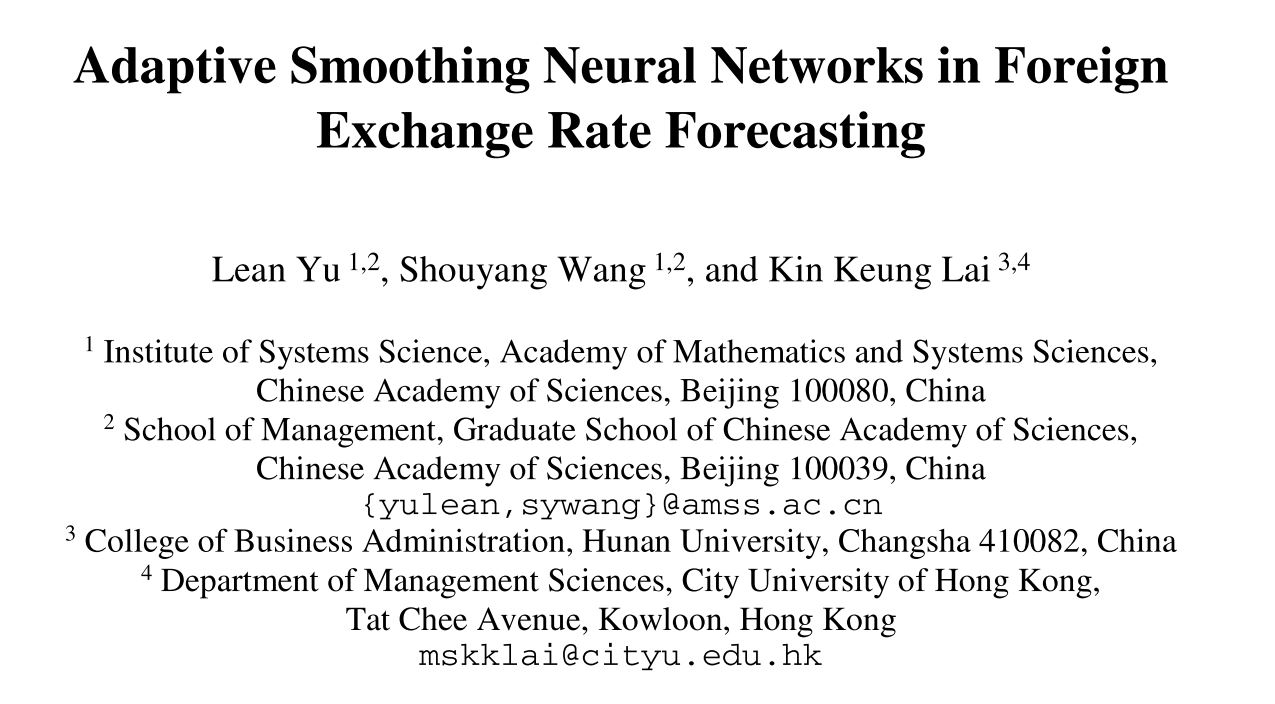
\includegraphics[width=3in]{003.jpg}
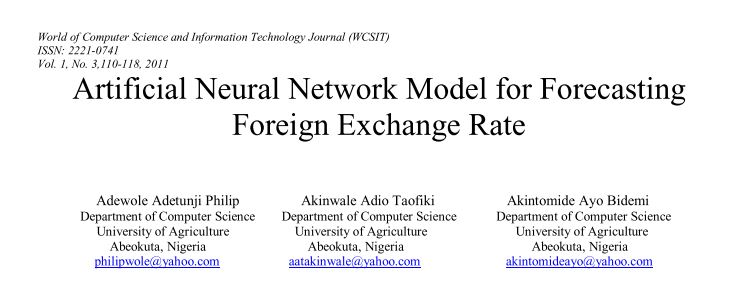
\includegraphics[width=3in]{002.jpg}

The first paper named "adaptive smoothing NN in FX forecasting". It indicates that Multi-Layer Feed-forward Network (MLFN)  is one of the best neural network structures, which could achieve a very high accuracy.

The second paper named "Artificial Neural Network Model for Forecasting Foreign Exchange Rate". This paper mentions Neuron Coefficient Smooth Transition Auto Regression (NCSTAR) algorithm , and it mentions The Hidden Markov Model (HMM). HMM is a pretty good idea for forecasting the forex rate. I'd like to spend some time on it  next.

\section{\H The study on NCSTAR}
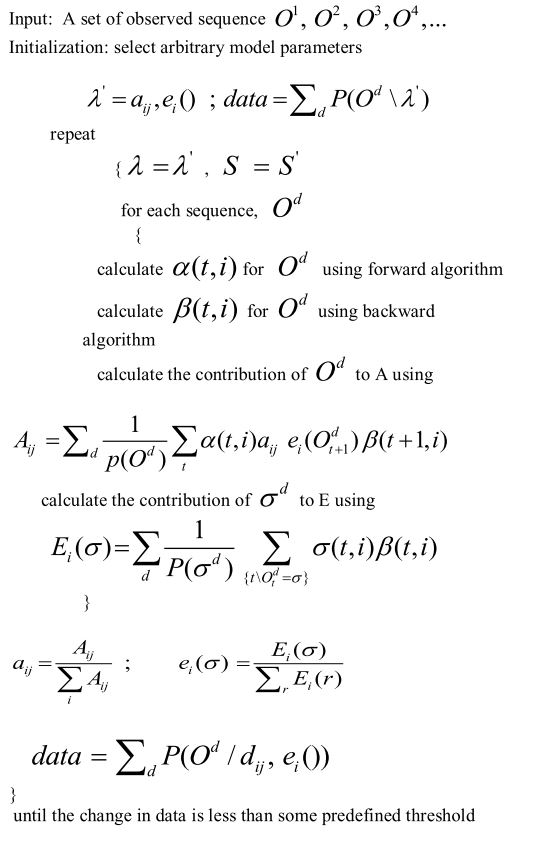
\includegraphics[width=4.5in]{001.jpg}









%%****************************************
%%  参考文献
%%****************************************
\bibliography{myreference}
\bibliographystyle{plain}
\end{document}  
